\documentclass[svgnames, 12pt]{beamer}

\usepackage[utf8]{inputenc}
\usepackage[english]{babel}
\usepackage[L7x]{fontenc}
\usepackage{lmodern}
\usepackage{amsmath}
\usepackage{amssymb}
\usepackage{xcolor}
\usepackage{subfig}
\usepackage{graphicx}
\usepackage{lipsum}
\usepackage{hyperref}

\definecolor{mifcolor}{RGB}{0, 71, 127}
\definecolor{dimgr}{RGB}{105, 105, 105}
\definecolor{sky}{RGB}{0, 191, 255}
\setbeamercolor{alerted text}{fg=red,bg=sky}
\newcommand{\boxalert}[1]{{%
	\usebeamercolor{alerted text}\colorbox{bg}{\alert{#1}}%
}}

\mode<presentation>{
\usetheme{Madrid}
\usecolortheme[named=mifcolor]{structure}
\setbeamertemplate{footline}
{%
	\leavevmode%
	\hbox{ \begin{beamercolorbox}[wd=.3\paperwidth,ht=2.5ex,dp=1.125ex,leftskip=.3cm
			plus1fill,rightskip=.3cm]{author in head/foot}%
			\usebeamerfont{author in head/foot}\insertshortauthor \hfill 
		\end{beamercolorbox}%
		\begin{beamercolorbox}[wd=.2\paperwidth,ht=2.5ex,dp=1.125ex,leftskip=.3cm,
			rightskip=.3cm plus1fil]{institute in head/foot}%
			\usebeamerfont{institute in head/foot}\insertshortinstitute
		\end{beamercolorbox}%
		\begin{beamercolorbox}[wd=.2\paperwidth,ht=2.5ex,dp=1.125ex,leftskip=.3cm,
			rightskip=.3cm plus1fil]{date in head/foot}%
			\usebeamerfont{date in head/foot}\insertshortdate
		\end{beamercolorbox}%
		\begin{beamercolorbox}[wd=.3\paperwidth,ht=2.5ex,dp=1.125ex,leftskip=.3cm,
			rightskip=.3cm plus1fil]{title in head/foot}%
			\usebeamerfont{title in head/foot}\insertshorttitle\hfill p.
			\insertframenumber\enspace of \inserttotalframenumber\enspace 
	\end{beamercolorbox} }%
	\vskip0pt%
}
}

\title[FDA of Weather Data]{Functional Data Analysis of Weather Data}%
\author[A. J. Smoliakov]{Aleksandr Jan Smoliakov\inst{1}}
\institute[VU MIF]{\inst{1} Vilnius University, Faculty of Mathematics and Informatics}
\date{2025--05--27}

\begin{document}

\begin{frame}

\includegraphics[scale=0.15]{MIF Garamond-logo.png} 
\hfill

\includegraphics[scale=0.15]{Logo_spalvotas.eps}

\titlepage
\end{frame}

\begin{frame}{Table of Contents}
\tableofcontents
\end{frame}

% --- RECAP SLIDE ---
\section{Data Source}

\begin{frame}{Data Source}
			\begin{itemize}
		\item \textbf{Historical Weather Data in India}
		\begin{itemize}
			\item Hourly observations (2006--2019)
			\item 8 major Indian cities
			\item Over 20 meteorological variables (focus on Temperature)
		\end{itemize}
			\end{itemize}
\end{frame}

\begin{frame}{Recap: Data, Smoothing, and Initial FPCA}
  \begin{itemize}
    \item \textbf{Data:} Hourly temperature data ($tempC$) for 8 Indian cities (2011-2018).
    \item \textbf{Preprocessing:}
        \begin{itemize}
            \item Data cleaned and augmented (day of year, hour of day).
            \item Averaged multi-year temperatures for each city, day of year, and hour of day, creating an average annual temperature surface (365 days $\times$ 24 hours) per city.
        \end{itemize}
    \item \textbf{Bivariate Smoothing:}
        \begin{itemize}
            \item Day dimension: B-spline basis (12 basis functions).
            \item Hour dimension: Fourier basis (11 basis functions, 5 harmonics + intercept).
            \item Optimal smoothing parameters ($\lambda_s = 0.001$, $\lambda_t = 10^{-5}$) selected via Generalized Cross-Validation (GCV).
            \item Result: Smoothed bivariate functional data object for each city's average temperature surface ($Y_{smoothed\_city\_avg}$). MAE $\approx 0.51^\circ C$.
        \end{itemize}
    \item \textbf{Initial FPCA (on City Averages):}
        \begin{itemize}
            \item Performed on the coefficients of the smoothed city-average surfaces.
            \item Revealed primary modes of variation in temperature patterns across cities.
            \item (You might have shown a plot of PC1 vs PC2 scores for cities here in your previous presentation).
        \end{itemize}
  \end{itemize}
  \pause
  \textbf{Today's Focus:} Deeper analysis building upon these smoothed functional representations.
\end{frame}

% --- DERIVATIVES ANALYSIS ---
\section{Derivatives Analysis}
\begin{frame}{Derivatives: Rates of Temperature Change}
  \framesubtitle{Understanding Dynamics for Bengaluru (Example City)}
  \begin{columns}[T] % Align columns at the top
    \begin{column}{0.5\textwidth}
      \textbf{Hourly Rate of Change ($\frac{\partial T}{\partial \text{hour}}$)}
      \begin{figure}
        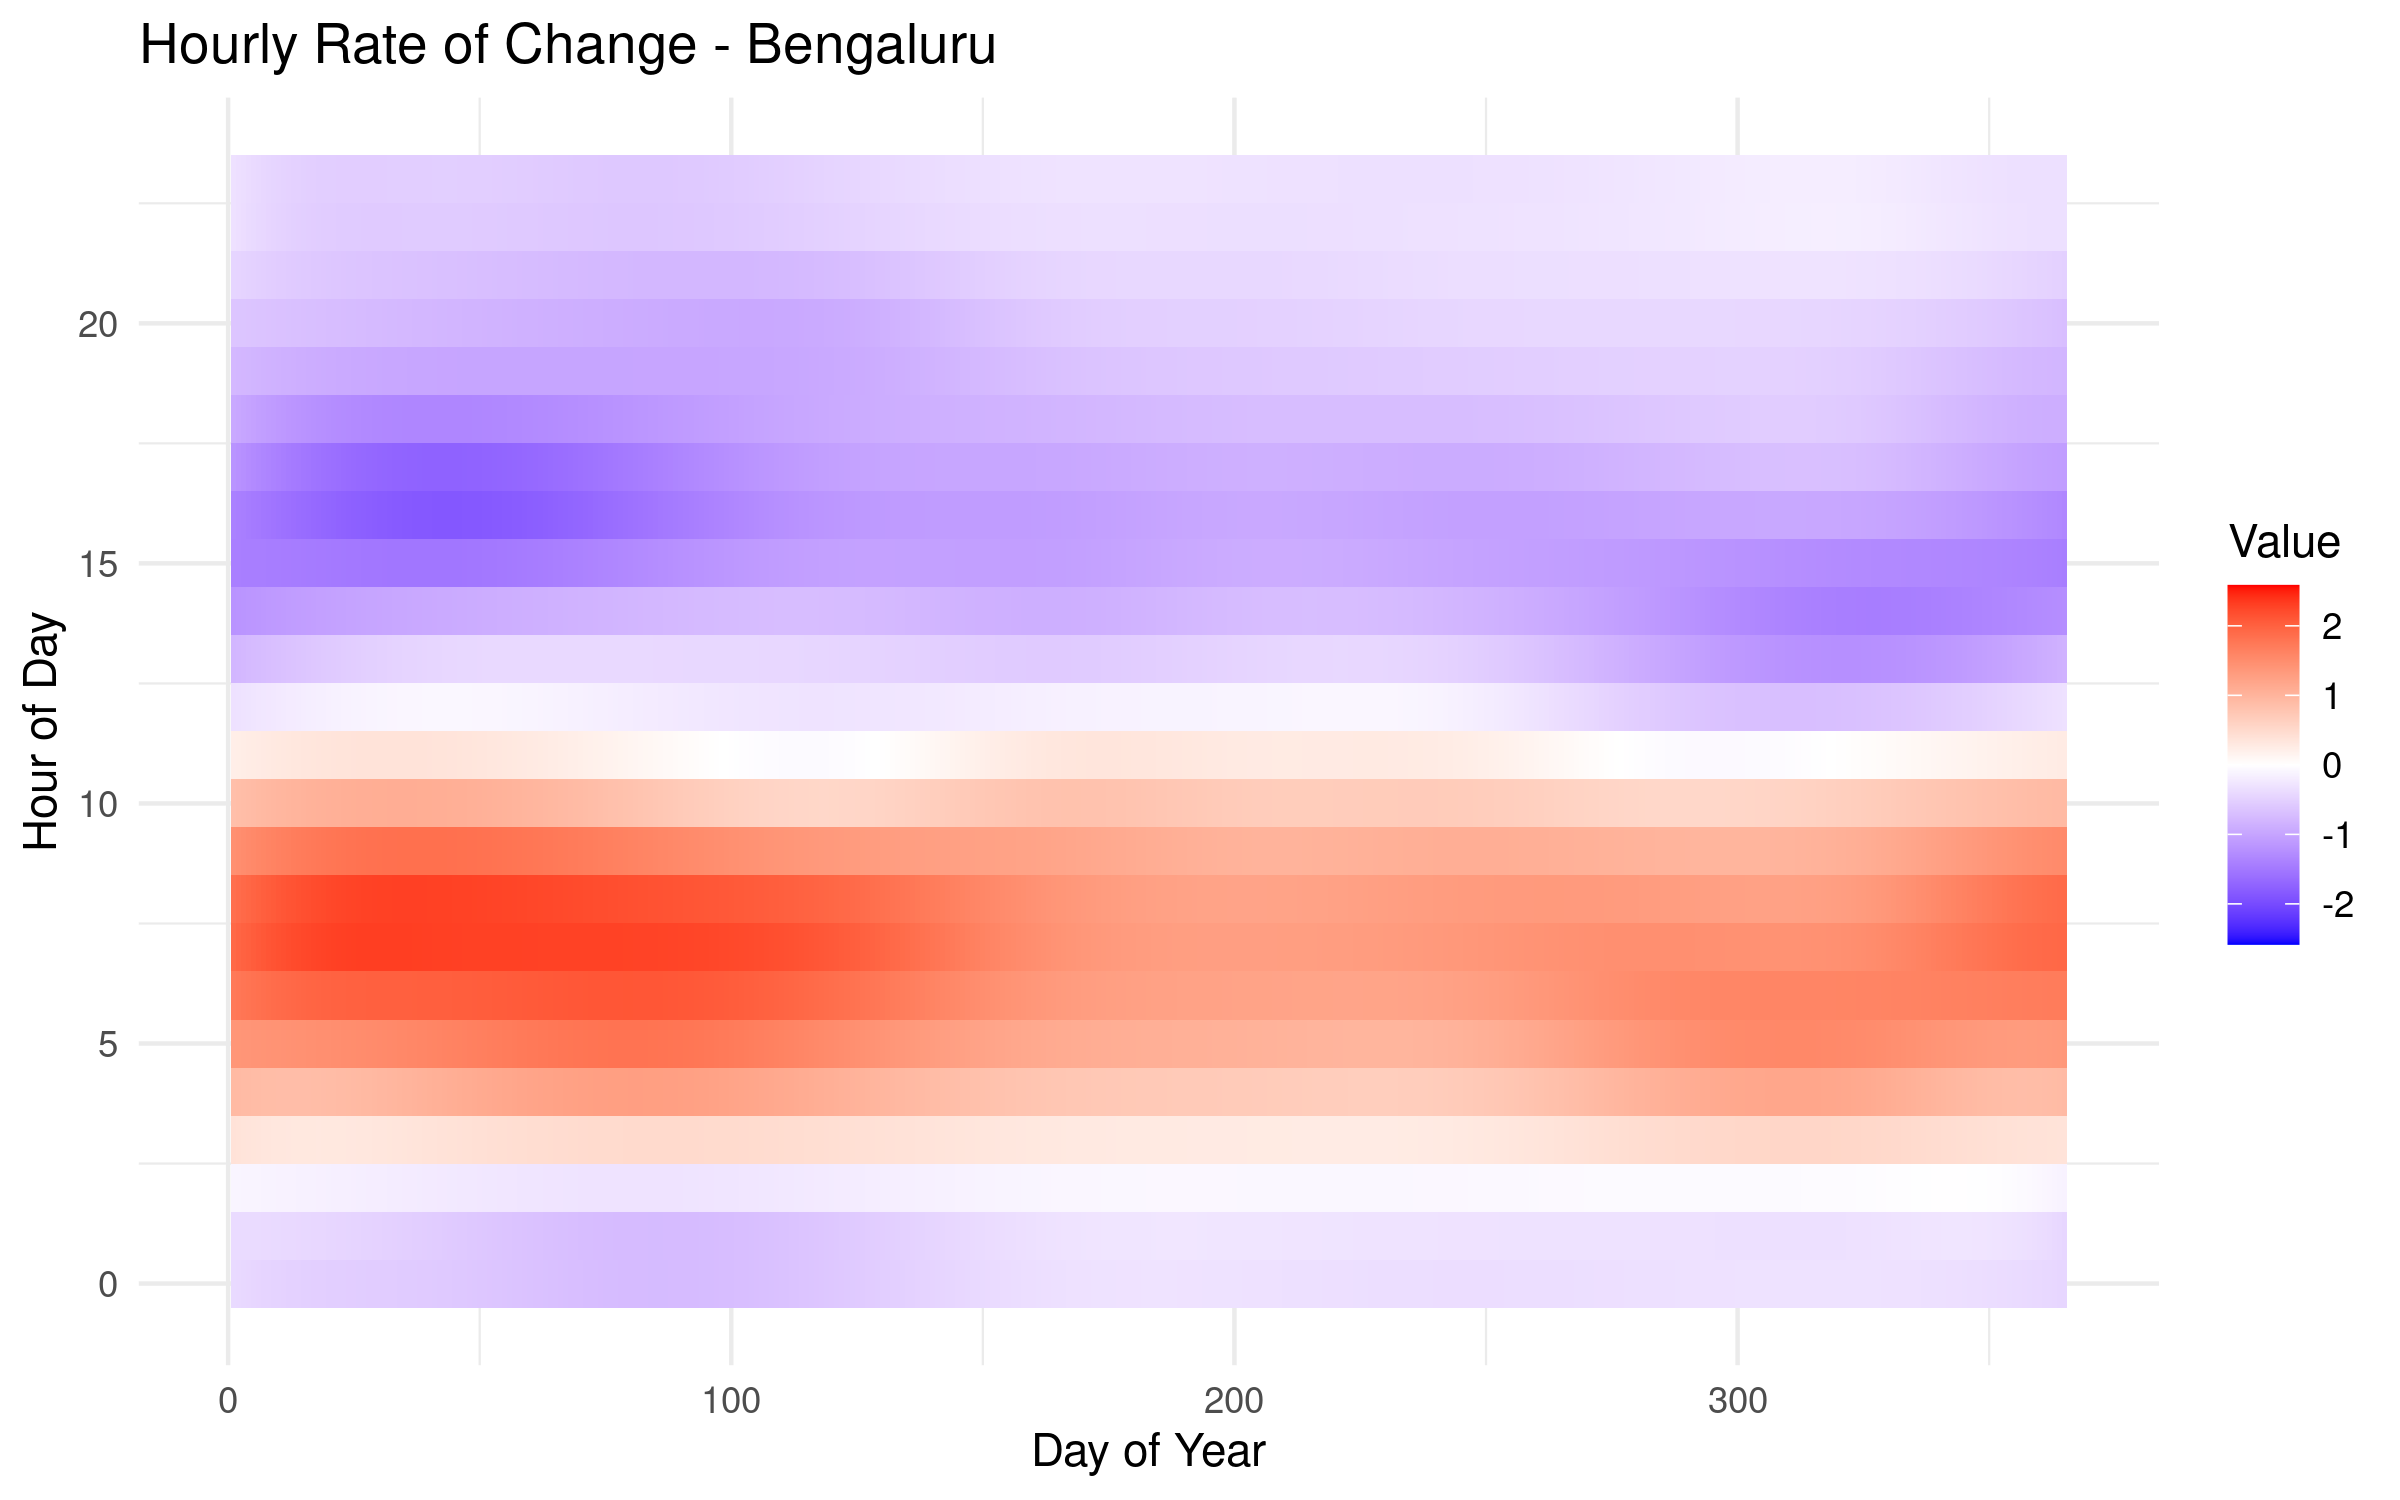
\includegraphics[width=\linewidth]{../data/output/figures/derivative_hour1_city_avg.png}
        \caption*{Rate of temperature change throughout the day, across the year. Red: warming, Blue: cooling.}
      \end{figure}
    \end{column}
    \begin{column}{0.5\textwidth}
      \textbf{Daily Rate of Change ($\frac{\partial T}{\partial \text{day}}$)}
      \begin{figure}
        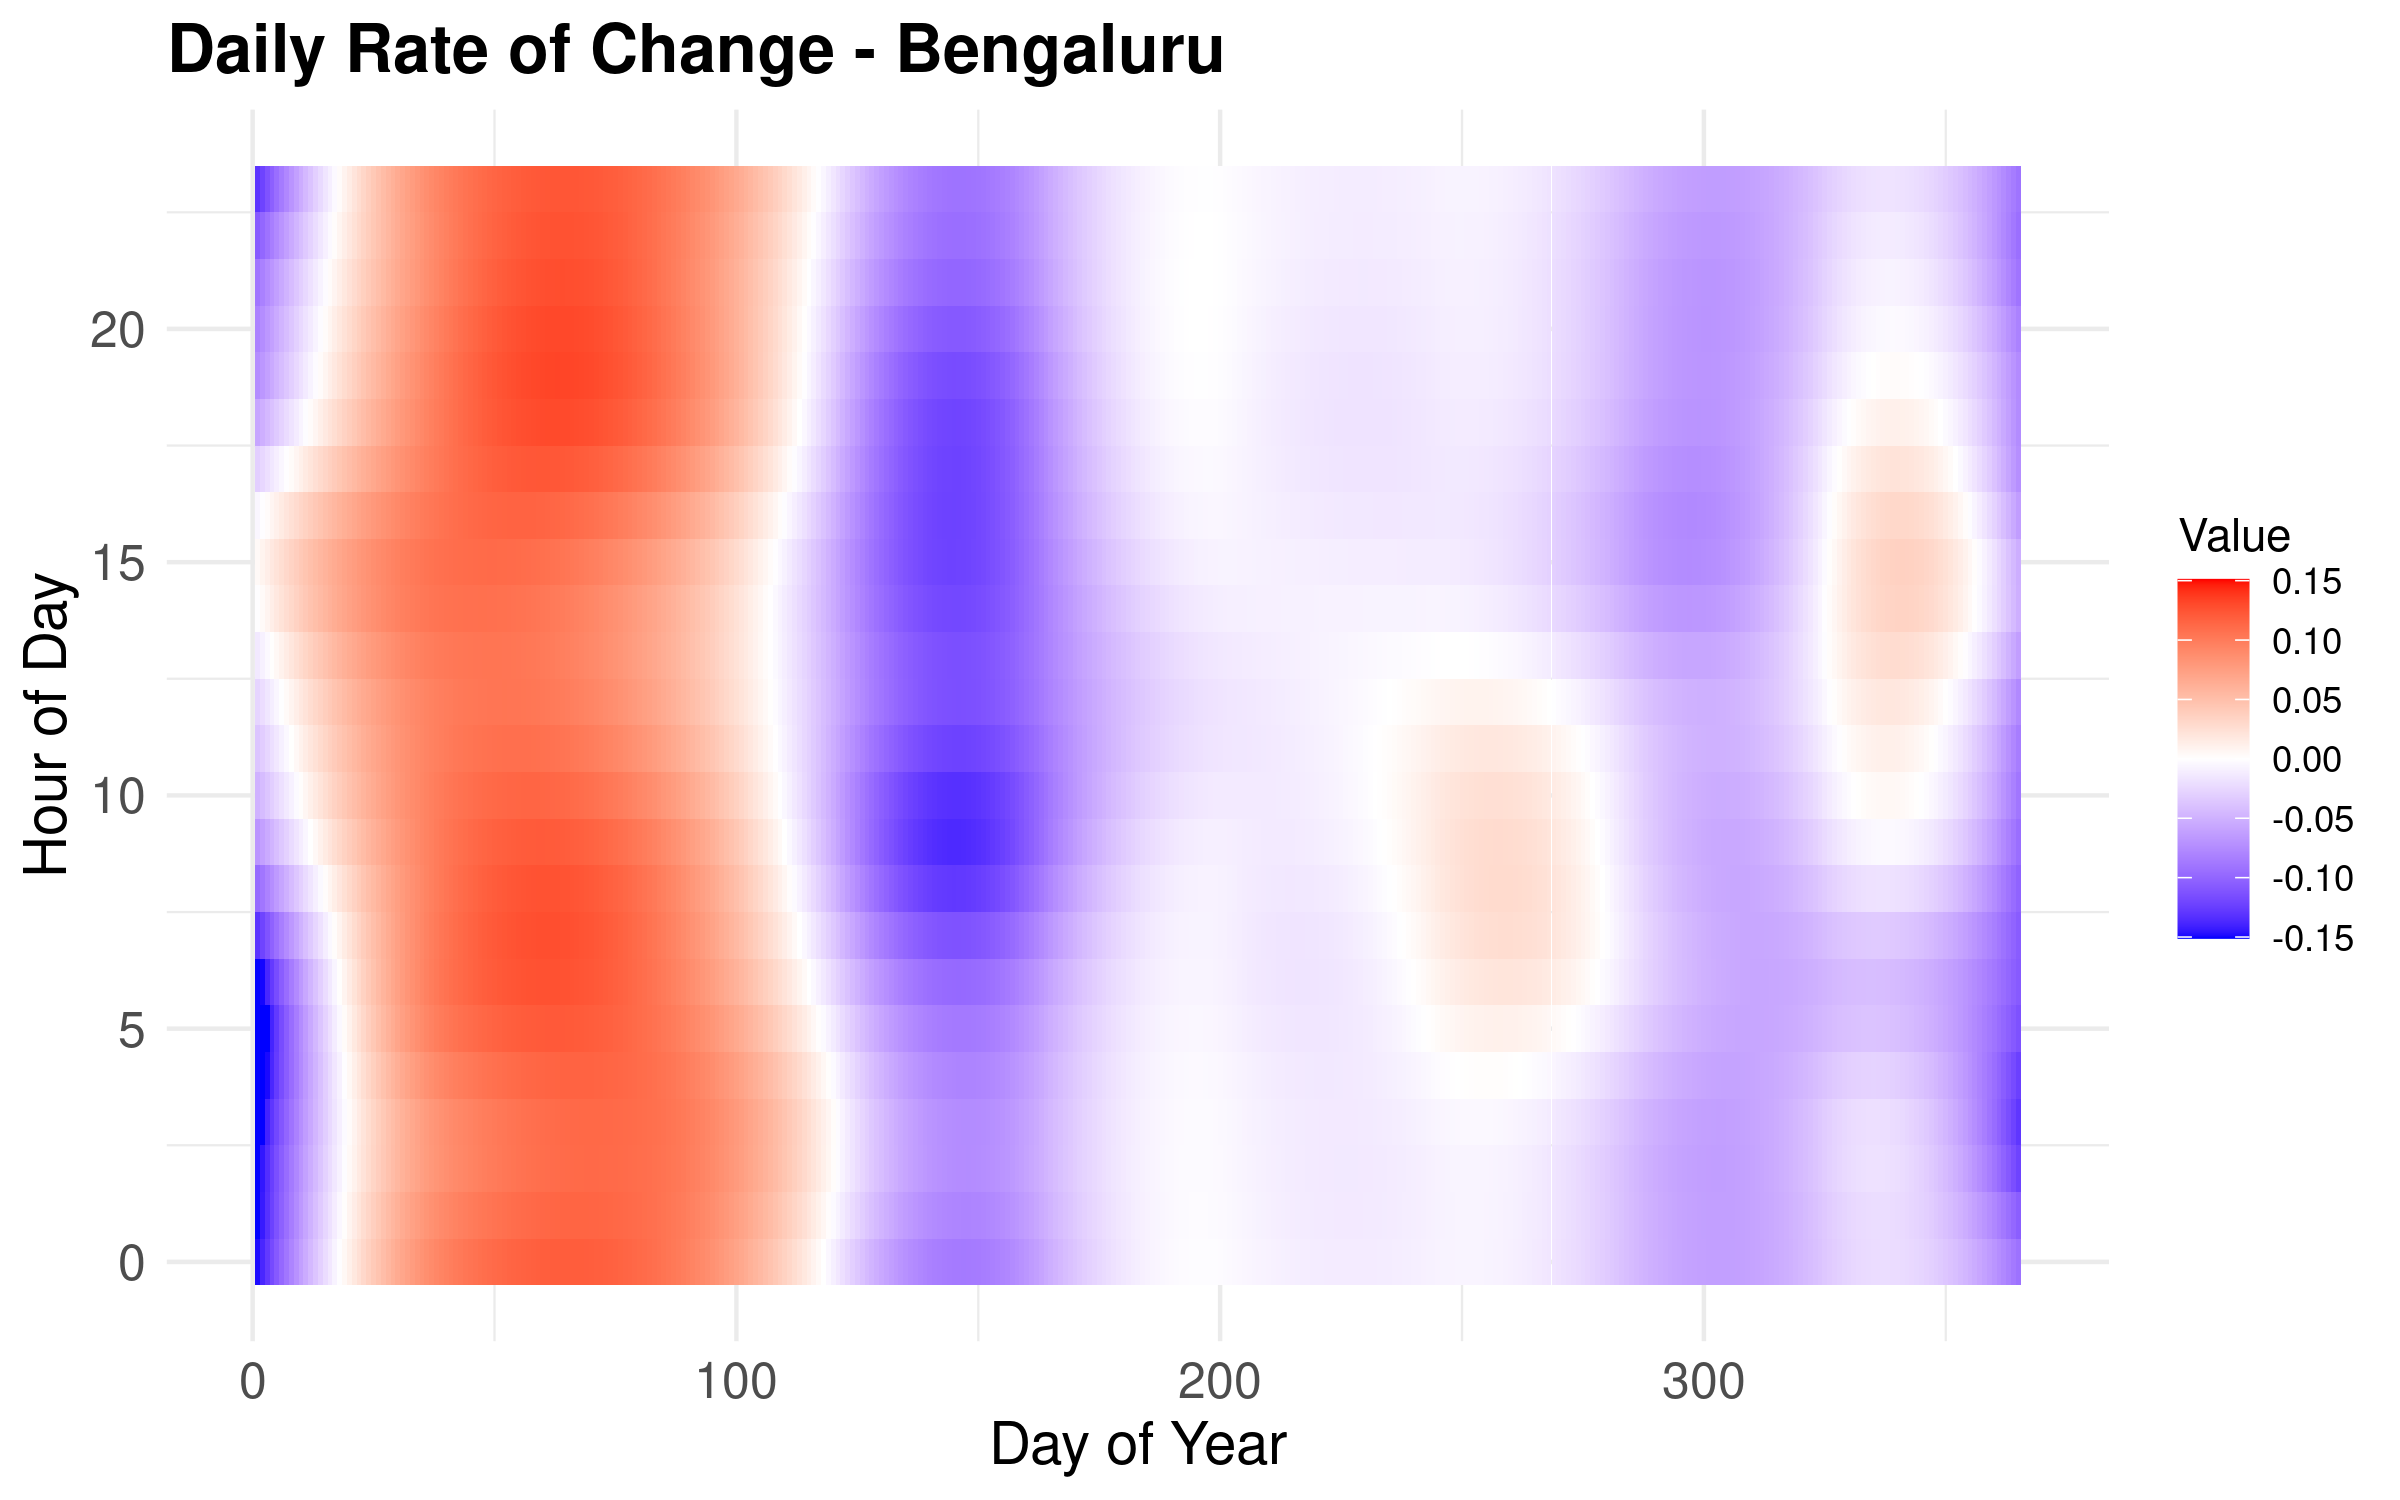
\includegraphics[width=\linewidth]{../data/output/figures/derivative_day1_city_avg.png}
        \caption*{Rate of temperature change from one day to the next, at different hours. Red: inter-day warming, Blue: inter-day cooling.}
      \end{figure}
    \end{column}
  \end{columns}
  \vspace{0.5em} % Small vertical space
  \textbf{Insights:}
  \begin{itemize}
    \item \textit{Hourly:} Clear diurnal patterns, e.g., rapid warming in morning, cooling in evening. Intensity varies seasonally.
    \item \textit{Daily:} Highlights periods of seasonal transitions (e.g., warming into summer, cooling into winter).
  \end{itemize}
\end{frame}

% --- COVARIANCE ANALYSIS ---
\section{Covariance Structure}
\begin{frame}{Covariance of Hourly Temperatures}
  \framesubtitle{For Bengaluru (Smoothed Daily Profiles as Replicates)}
  \begin{figure}
    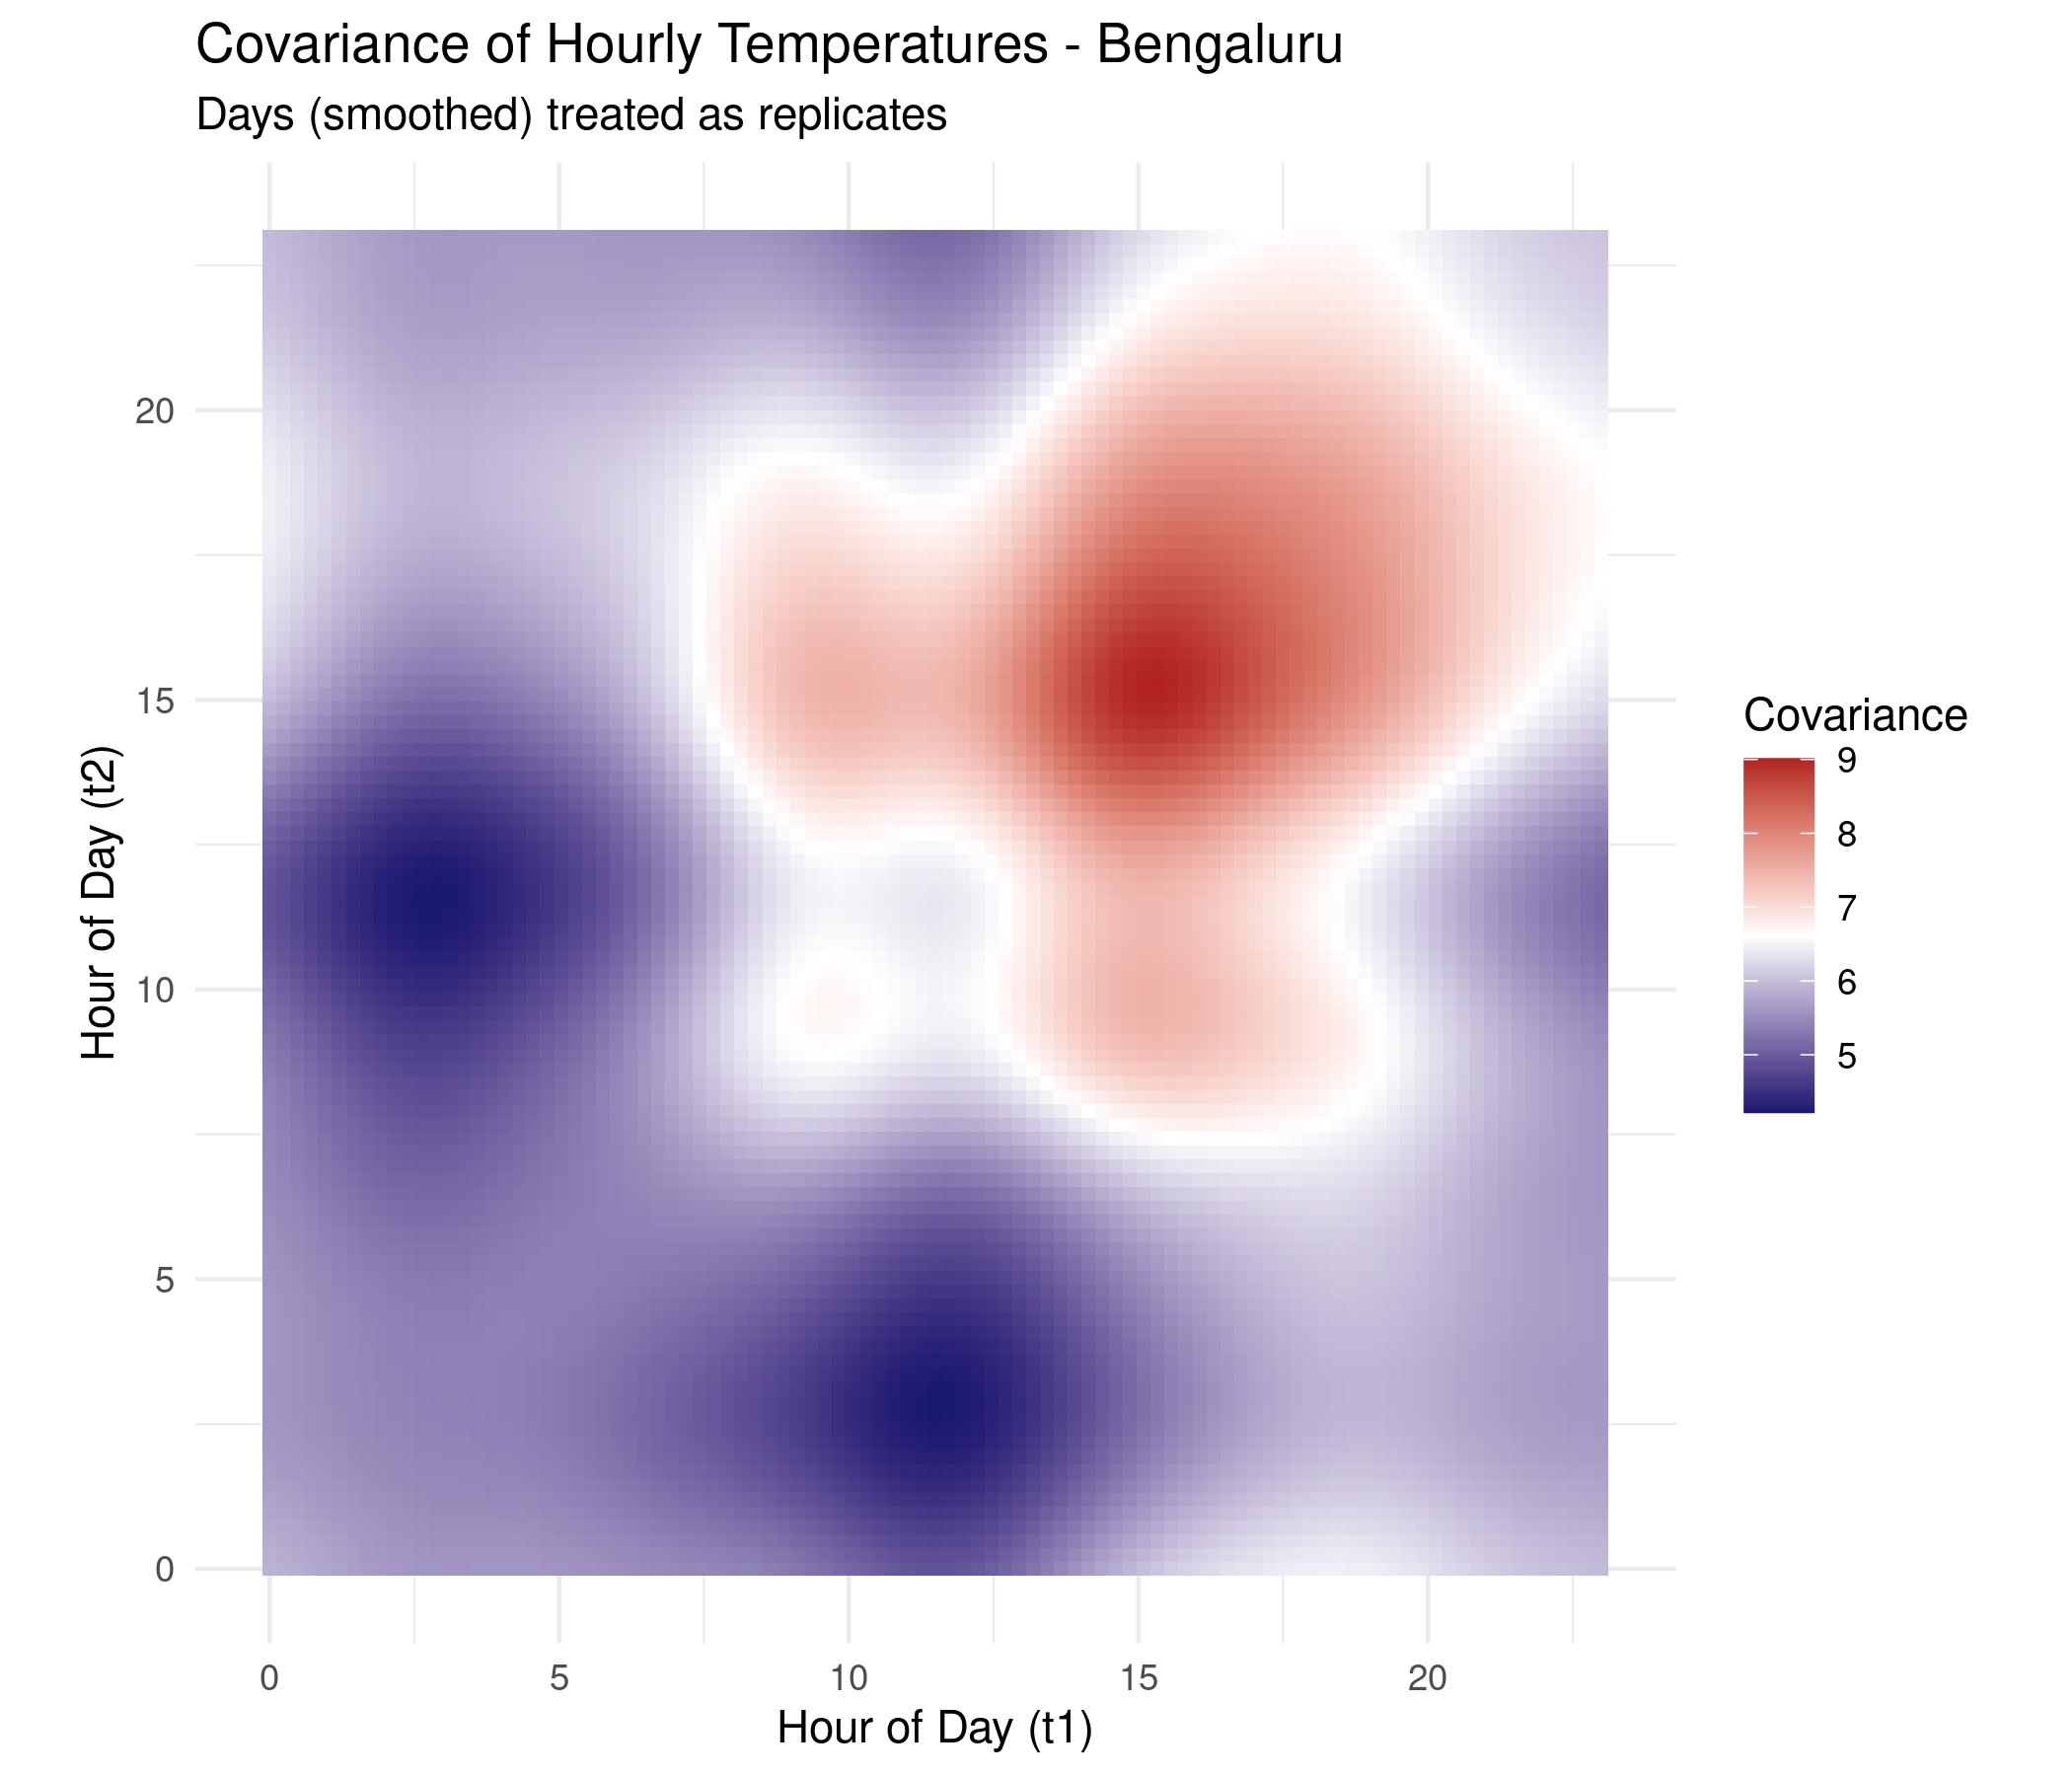
\includegraphics[width=0.7\linewidth]{../data/output/figures/covariance_heatmap_hourly_city_avg.png}
    \caption{Covariance: $Cov(T(t_1), T(t_2))$. High positive covariance (red) means temperatures at $t_1$ and $t_2$ tend to be high/low together.}
  \end{figure}
  \textbf{Interpretation:}
  \begin{itemize}
    \item Strong positive covariance between nearby hours, as expected.
    \item Covariance structure reveals how temperatures at different times of day co-vary.
    \item E.g., midday temperatures are highly correlated with afternoon temperatures. Morning and evening temperatures might be less correlated.
  \end{itemize}
\end{frame}

% --- FPCA ON YEARLY DATA ---
\section{FPCA on Yearly Data}
\begin{frame}{FPCA on Yearly Temperature Surfaces}
  \framesubtitle{Each City-Year Combination as a Replicate (64 surfaces)}
  \textbf{Objective:} Explore inter-annual variability and city-specific temporal trends.
  \begin{itemize}
    \item Yearly temperature surfaces (365 days $\times$ 24 hours) for each city and each year (2011-2018) were smoothed.
    \item FPCA performed on the coefficients of these 64 smoothed surfaces.
  \end{itemize}
  \begin{figure}
    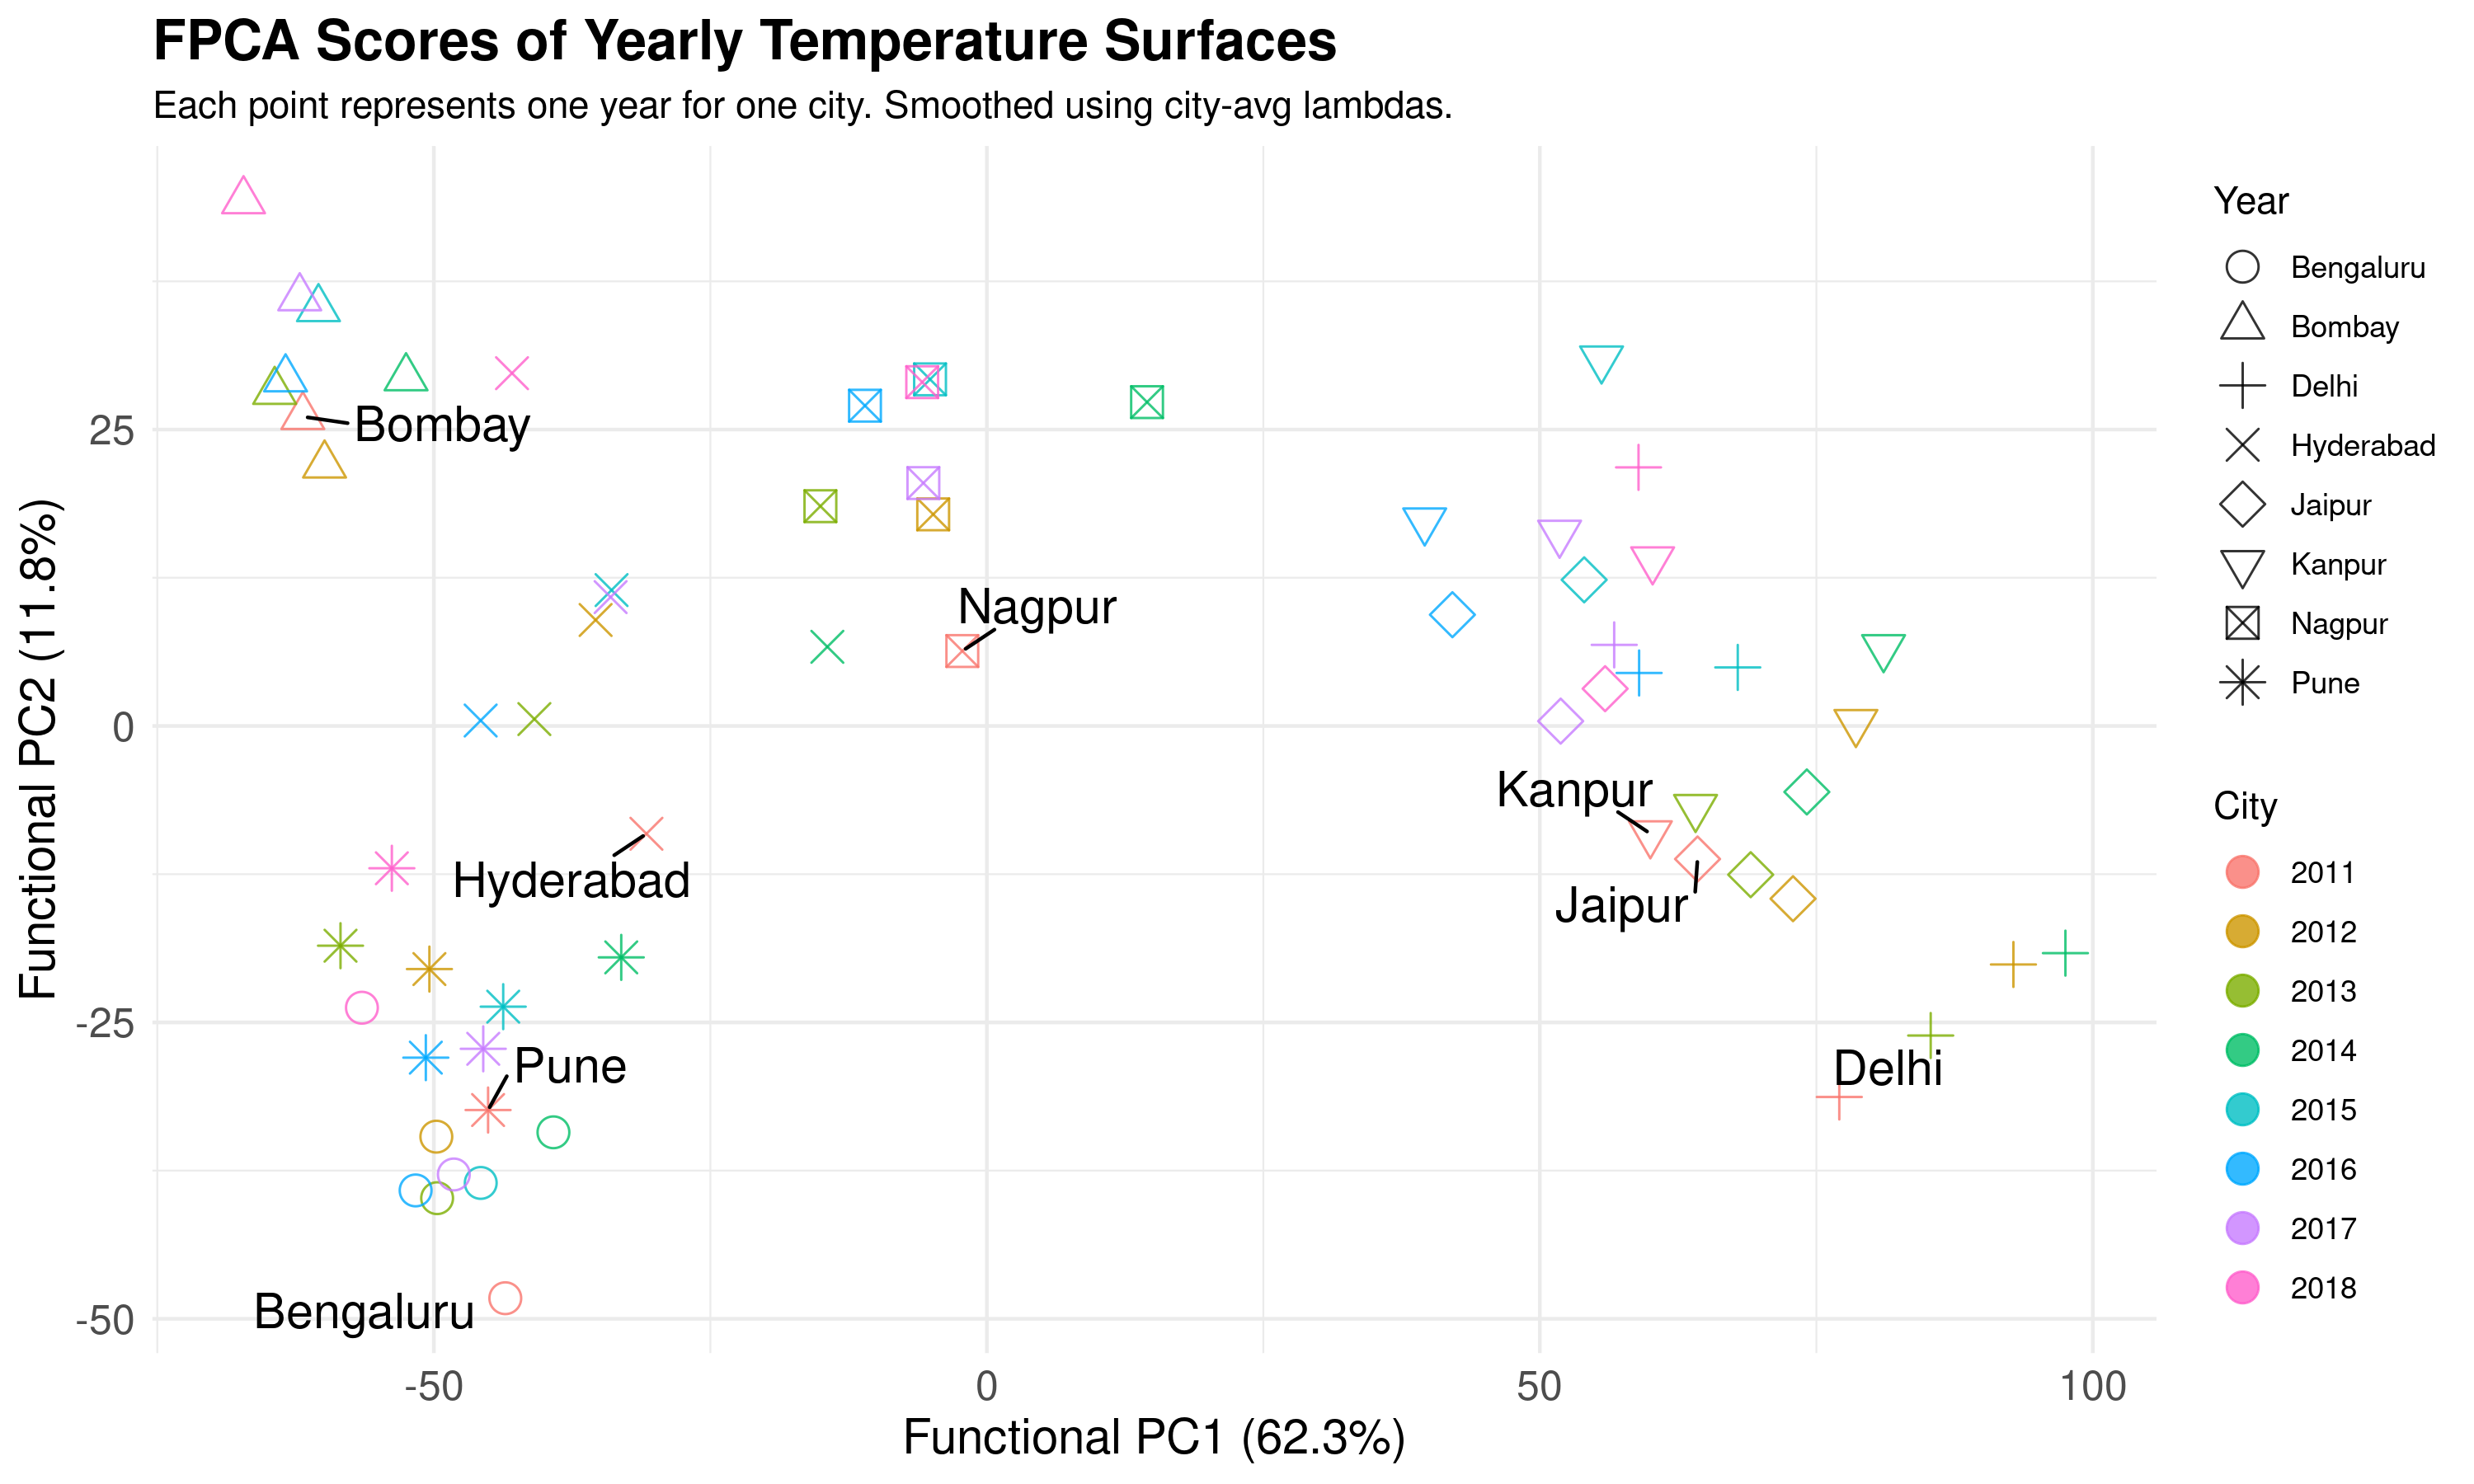
\includegraphics[width=0.9\linewidth]{../data/output/figures/pca_yearly_scores.png}
    \caption{FPCA Scores (PC1 vs PC2) for Yearly Surfaces. Colors: Year, Shapes: City.}
  \end{figure}
  \textbf{Key Observations:}
  \begin{itemize}
    \item \textit{PC1 (X-axis, explains X.X\% Var):} Likely captures overall annual mean temperature or amplitude.
    \item \textit{PC2 (Y-axis, explains Y.Y\% Var):} Might represent phase shifts or differences in seasonal shape.
    \item Points for the same city (same shape) show year-to-year variations.
    \item Different cities occupy distinct regions, indicating unique baseline climate patterns.
  \end{itemize}
  \textit{(Update X.X\% with actual variance explained values from your notebook for PC1 and PC2).}
\end{frame}

% --- CLUSTERING ANALYSIS ---
\section{Clustering of Cities}
\begin{frame}{Clustering Cities by Average Temperature Profiles}
  \framesubtitle{Based on FPCA Scores from City-Average Surfaces}
  \begin{itemize}
    \item Hierarchical clustering (Ward.D2 method) on PC1, PC2, PC3 scores of the 8 city-average temperature surfaces.
    \item A chosen number of $k=2$ clusters was selected.
  \end{itemize}
  \begin{columns}[T]
    \begin{column}{0.5\textwidth}
      \textbf{Clusters in PCA Space (PC1 vs PC2)}
      \begin{figure}
        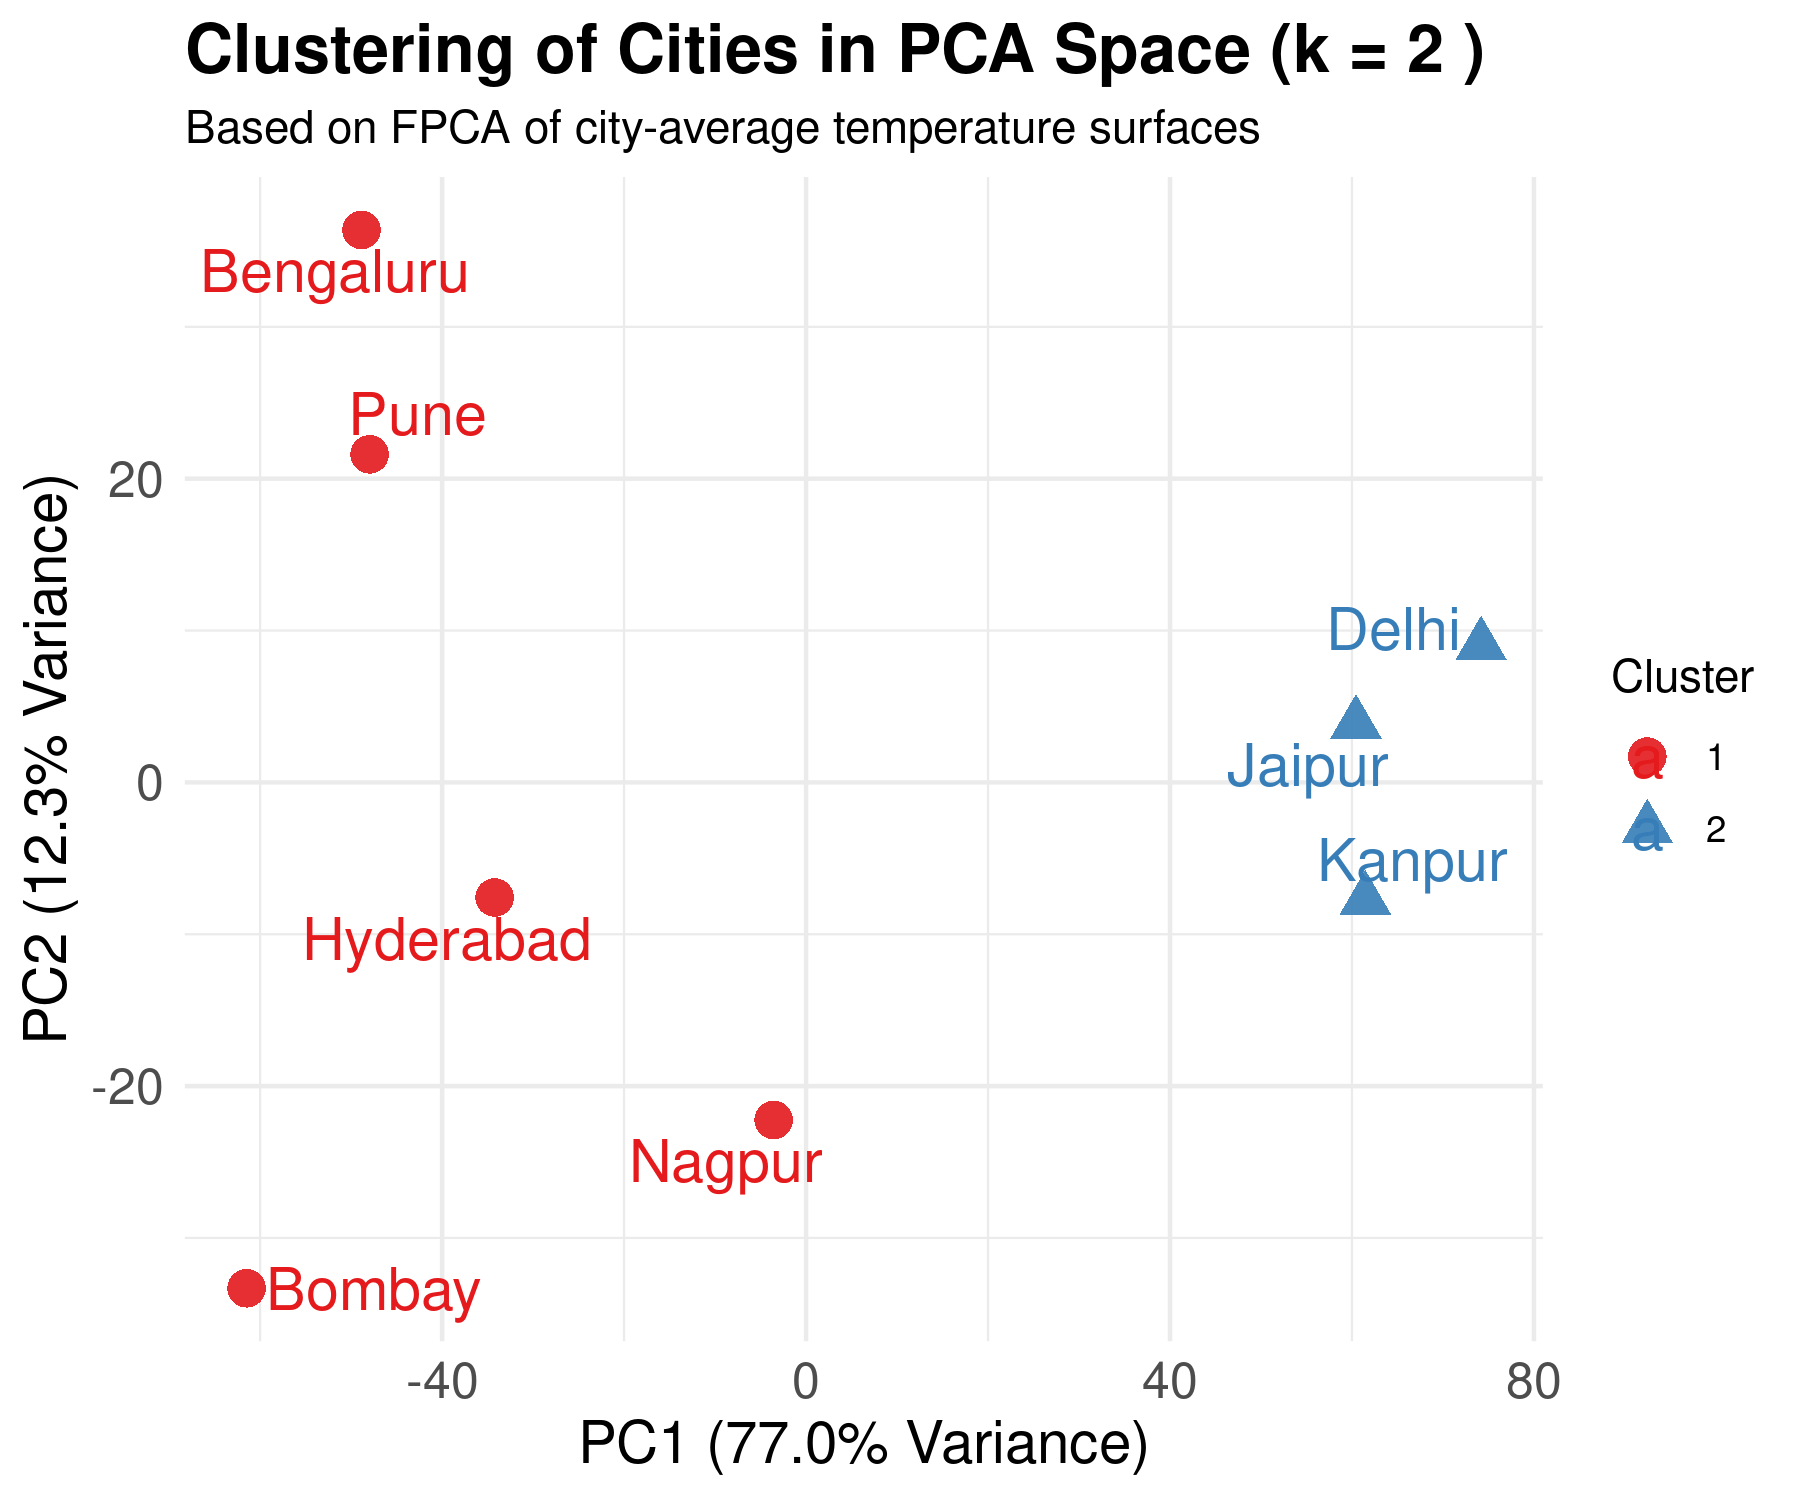
\includegraphics[width=\linewidth]{../data/output/figures/pca_clusters_city_avg.png}
      \end{figure}
    \end{column}
    \begin{column}{0.5\textwidth}
      \textbf{Geographical Distribution of Clusters}
      \begin{figure}
        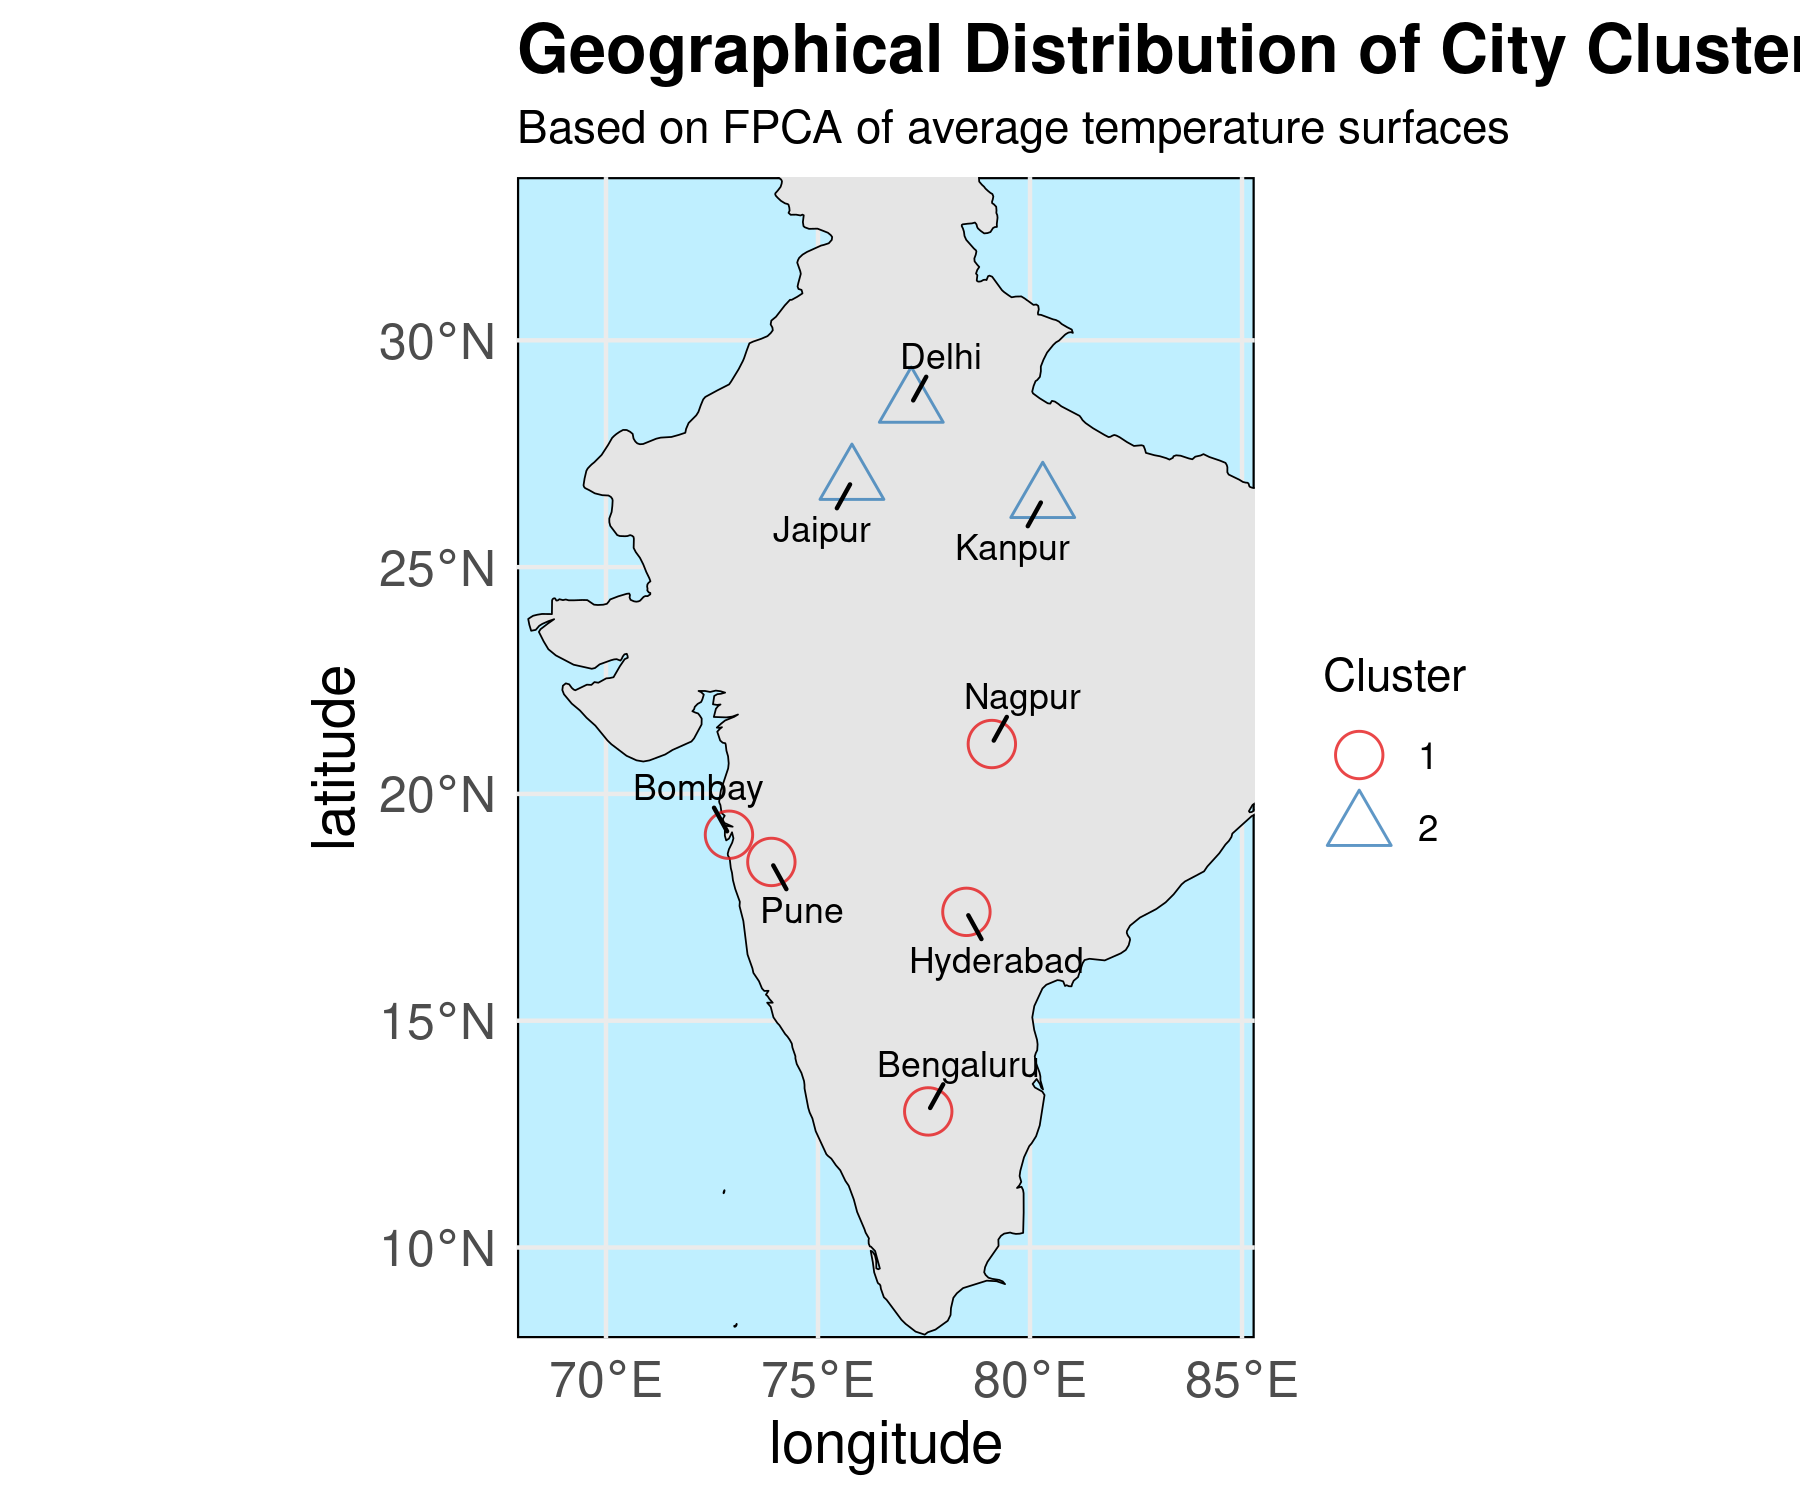
\includegraphics[width=\linewidth]{../data/output/figures/cluster_map_india.png}
      \end{figure}
    \end{column}
  \end{columns}
  \textbf{Identified Clusters:}
  \begin{itemize}
    \item \textit{Cluster 1:} Bengaluru, Bombay, Hyderabad, Nagpur, Pune (Southern/Central, Coastal/Peninsular).
    \item \textit{Cluster 2:} Delhi, Jaipur, Kanpur (Northern/Inland).
  \end{itemize}
\end{frame}

% --- CLUSTER COMPARISON ---
\begin{frame}{Comparing Cluster Characteristics}
  \framesubtitle{Mean Temperature Surfaces per Cluster}
  \begin{columns}[T]
    \begin{column}{0.5\textwidth}
      \textbf{Mean Surface - Cluster 1}
      \begin{figure}
        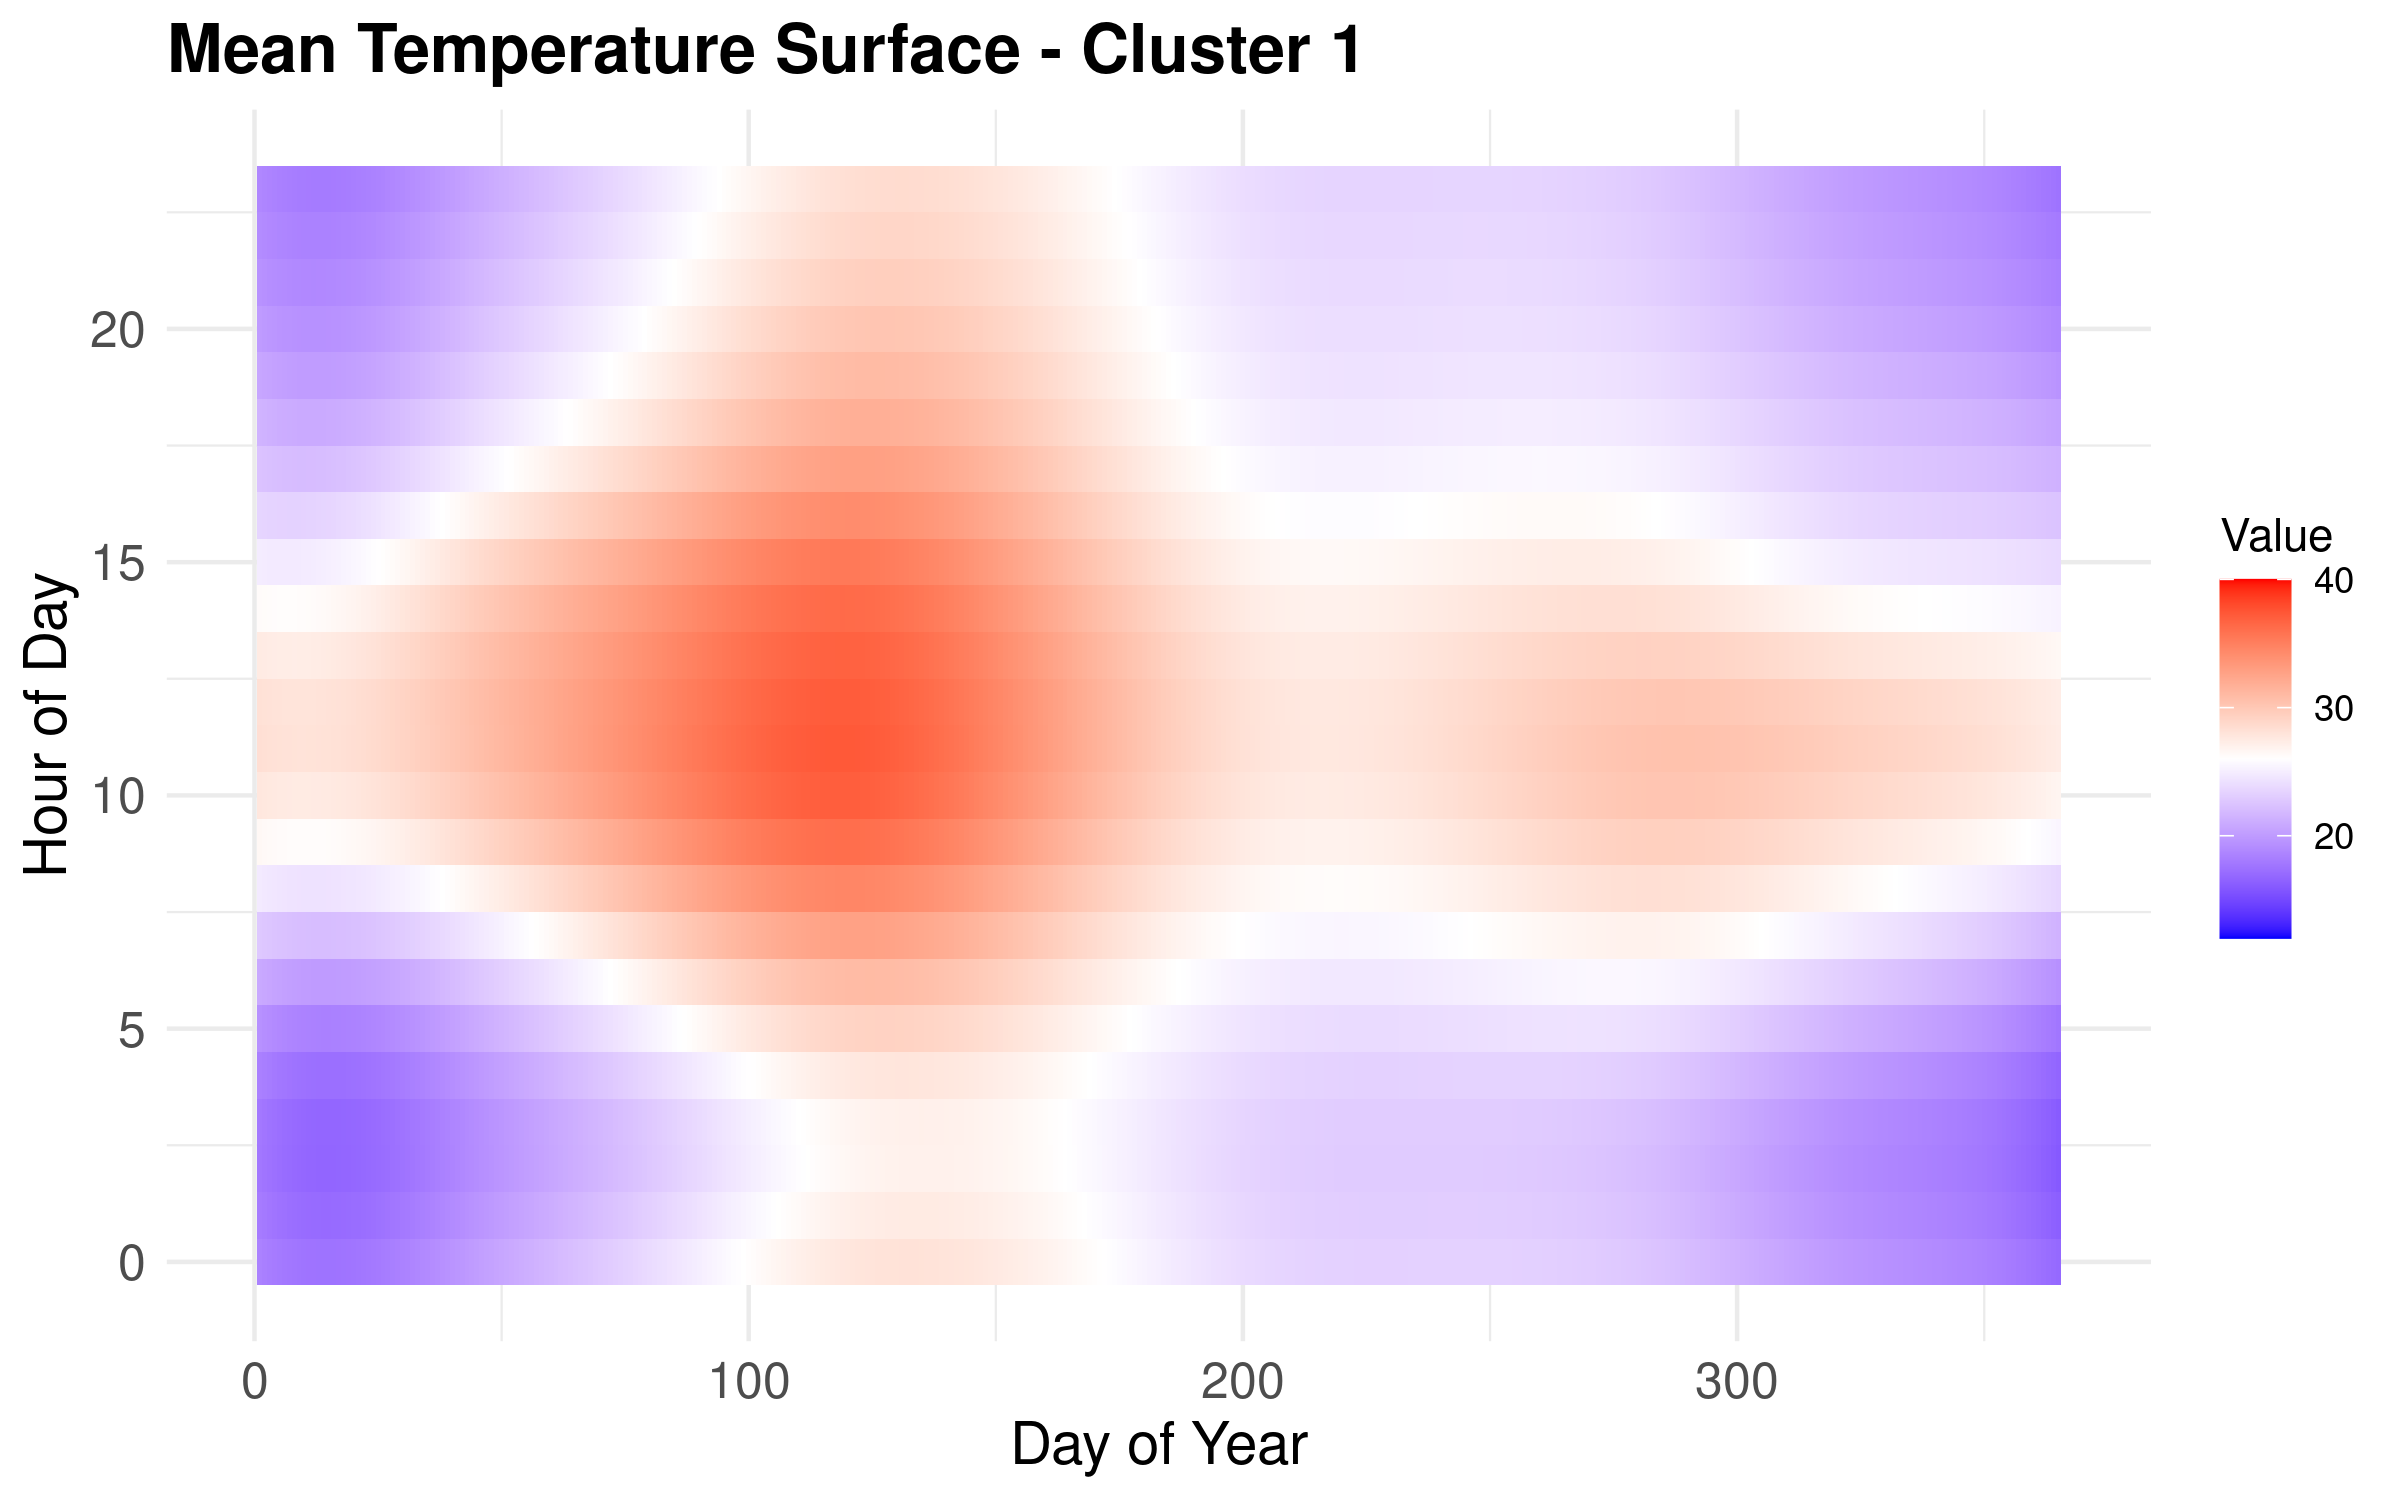
\includegraphics[width=\linewidth]{../data/output/figures/mean_surface_cluster_1.png}
        \caption*{\tiny Cities: Bengaluru, Bombay, Hyderabad, Nagpur, Pune.}
      \end{figure}
    \end{column}
    \begin{column}{0.5\textwidth}
      \textbf{Mean Surface - Cluster 2}
      \begin{figure}
        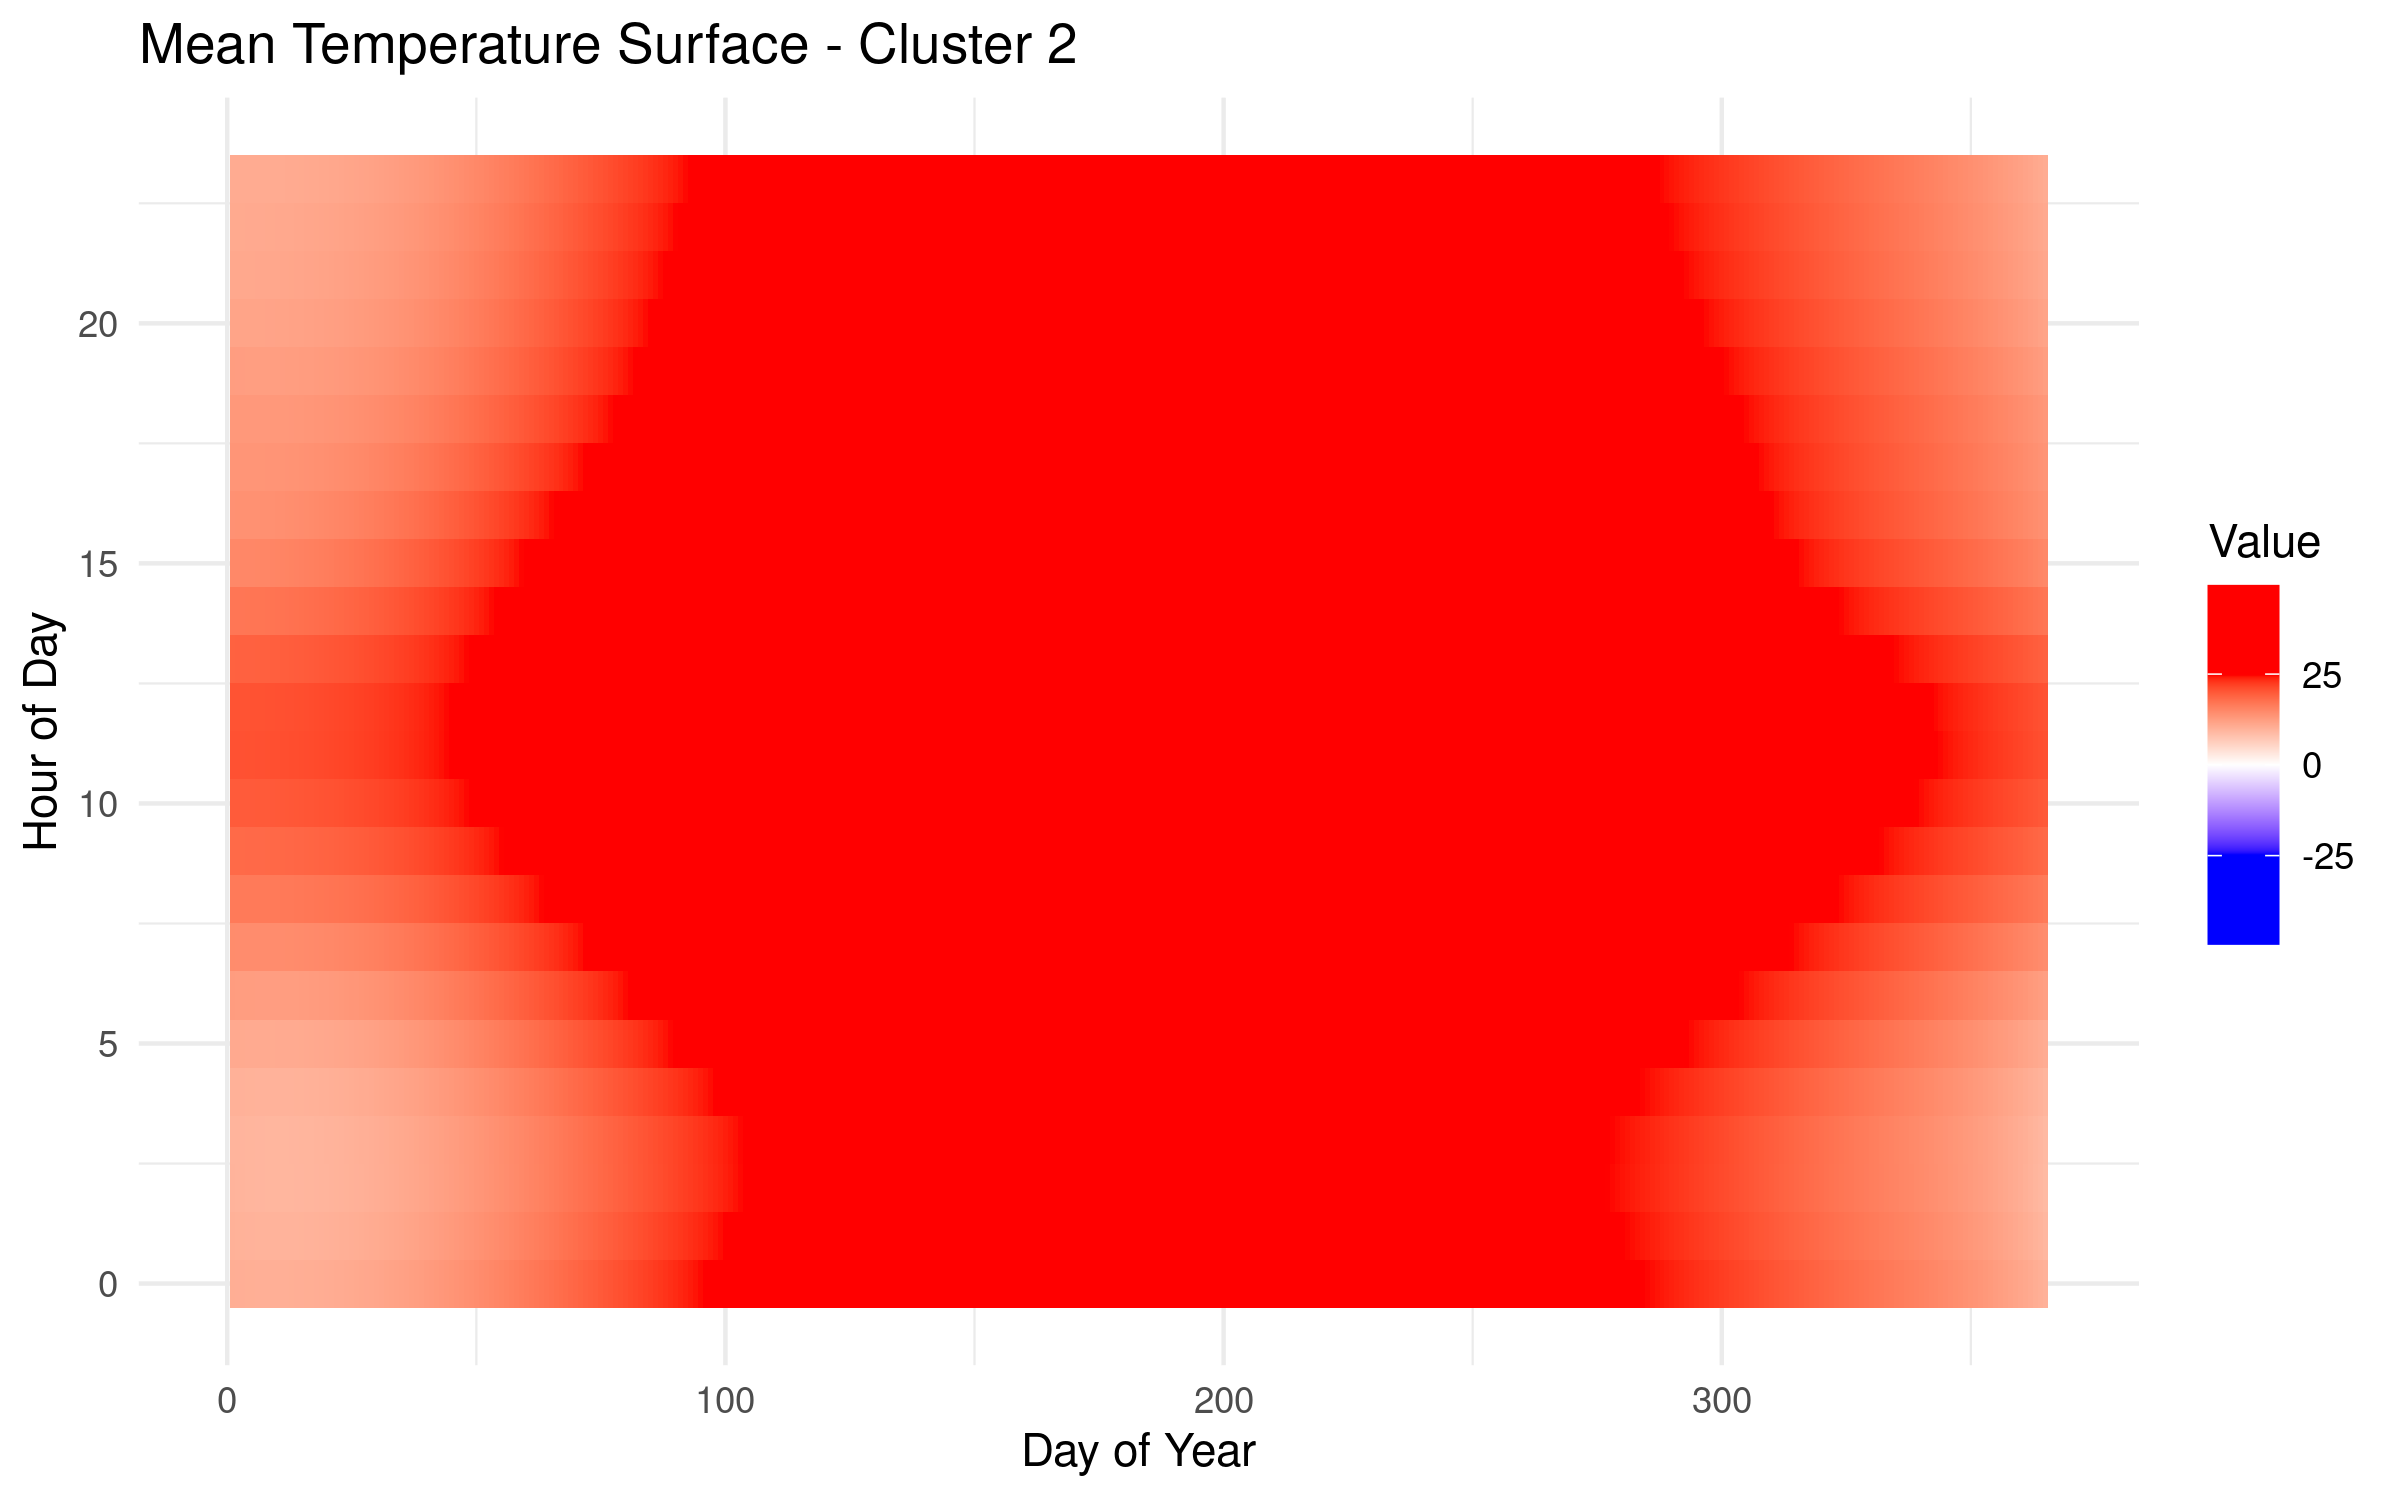
\includegraphics[width=\linewidth]{../data/output/figures/mean_surface_cluster_2.png}
        \caption*{\tiny Cities: Delhi, Jaipur, Kanpur.}
      \end{figure}
    \end{column}
  \end{columns}
  \textbf{Observations:}
  \begin{itemize}
    \item \textbf{Cluster 1 (Southern/Central):} Generally warmer winters, less extreme summer highs, possibly more influence from monsoonal patterns affecting daily temperature ranges.
    \item \textbf{Cluster 2 (Northern/Inland):} More pronounced seasonality with colder winters and hotter summers. Greater diurnal temperature range, especially outside monsoon.
    \item Differences visible in overall temperature levels and the timing/intensity of seasons.
  \end{itemize}
\end{frame}

% --- POINTWISE FANOVA ---
\section{Significance of Cluster Differences}
\begin{frame}{Pointwise FANOVA: Significance of Temperature Differences}
  \framesubtitle{Testing $H_0$: Mean Temp Surface is Same for Both Clusters}
  \begin{itemize}
    \item For each day of year and hour of day, an ANOVA was performed: $Temperature \sim Cluster$.
    \item The heatmap shows the $-\log_{10}(\text{p-value})$ for the cluster effect.
  \end{itemize}
  \begin{figure}
    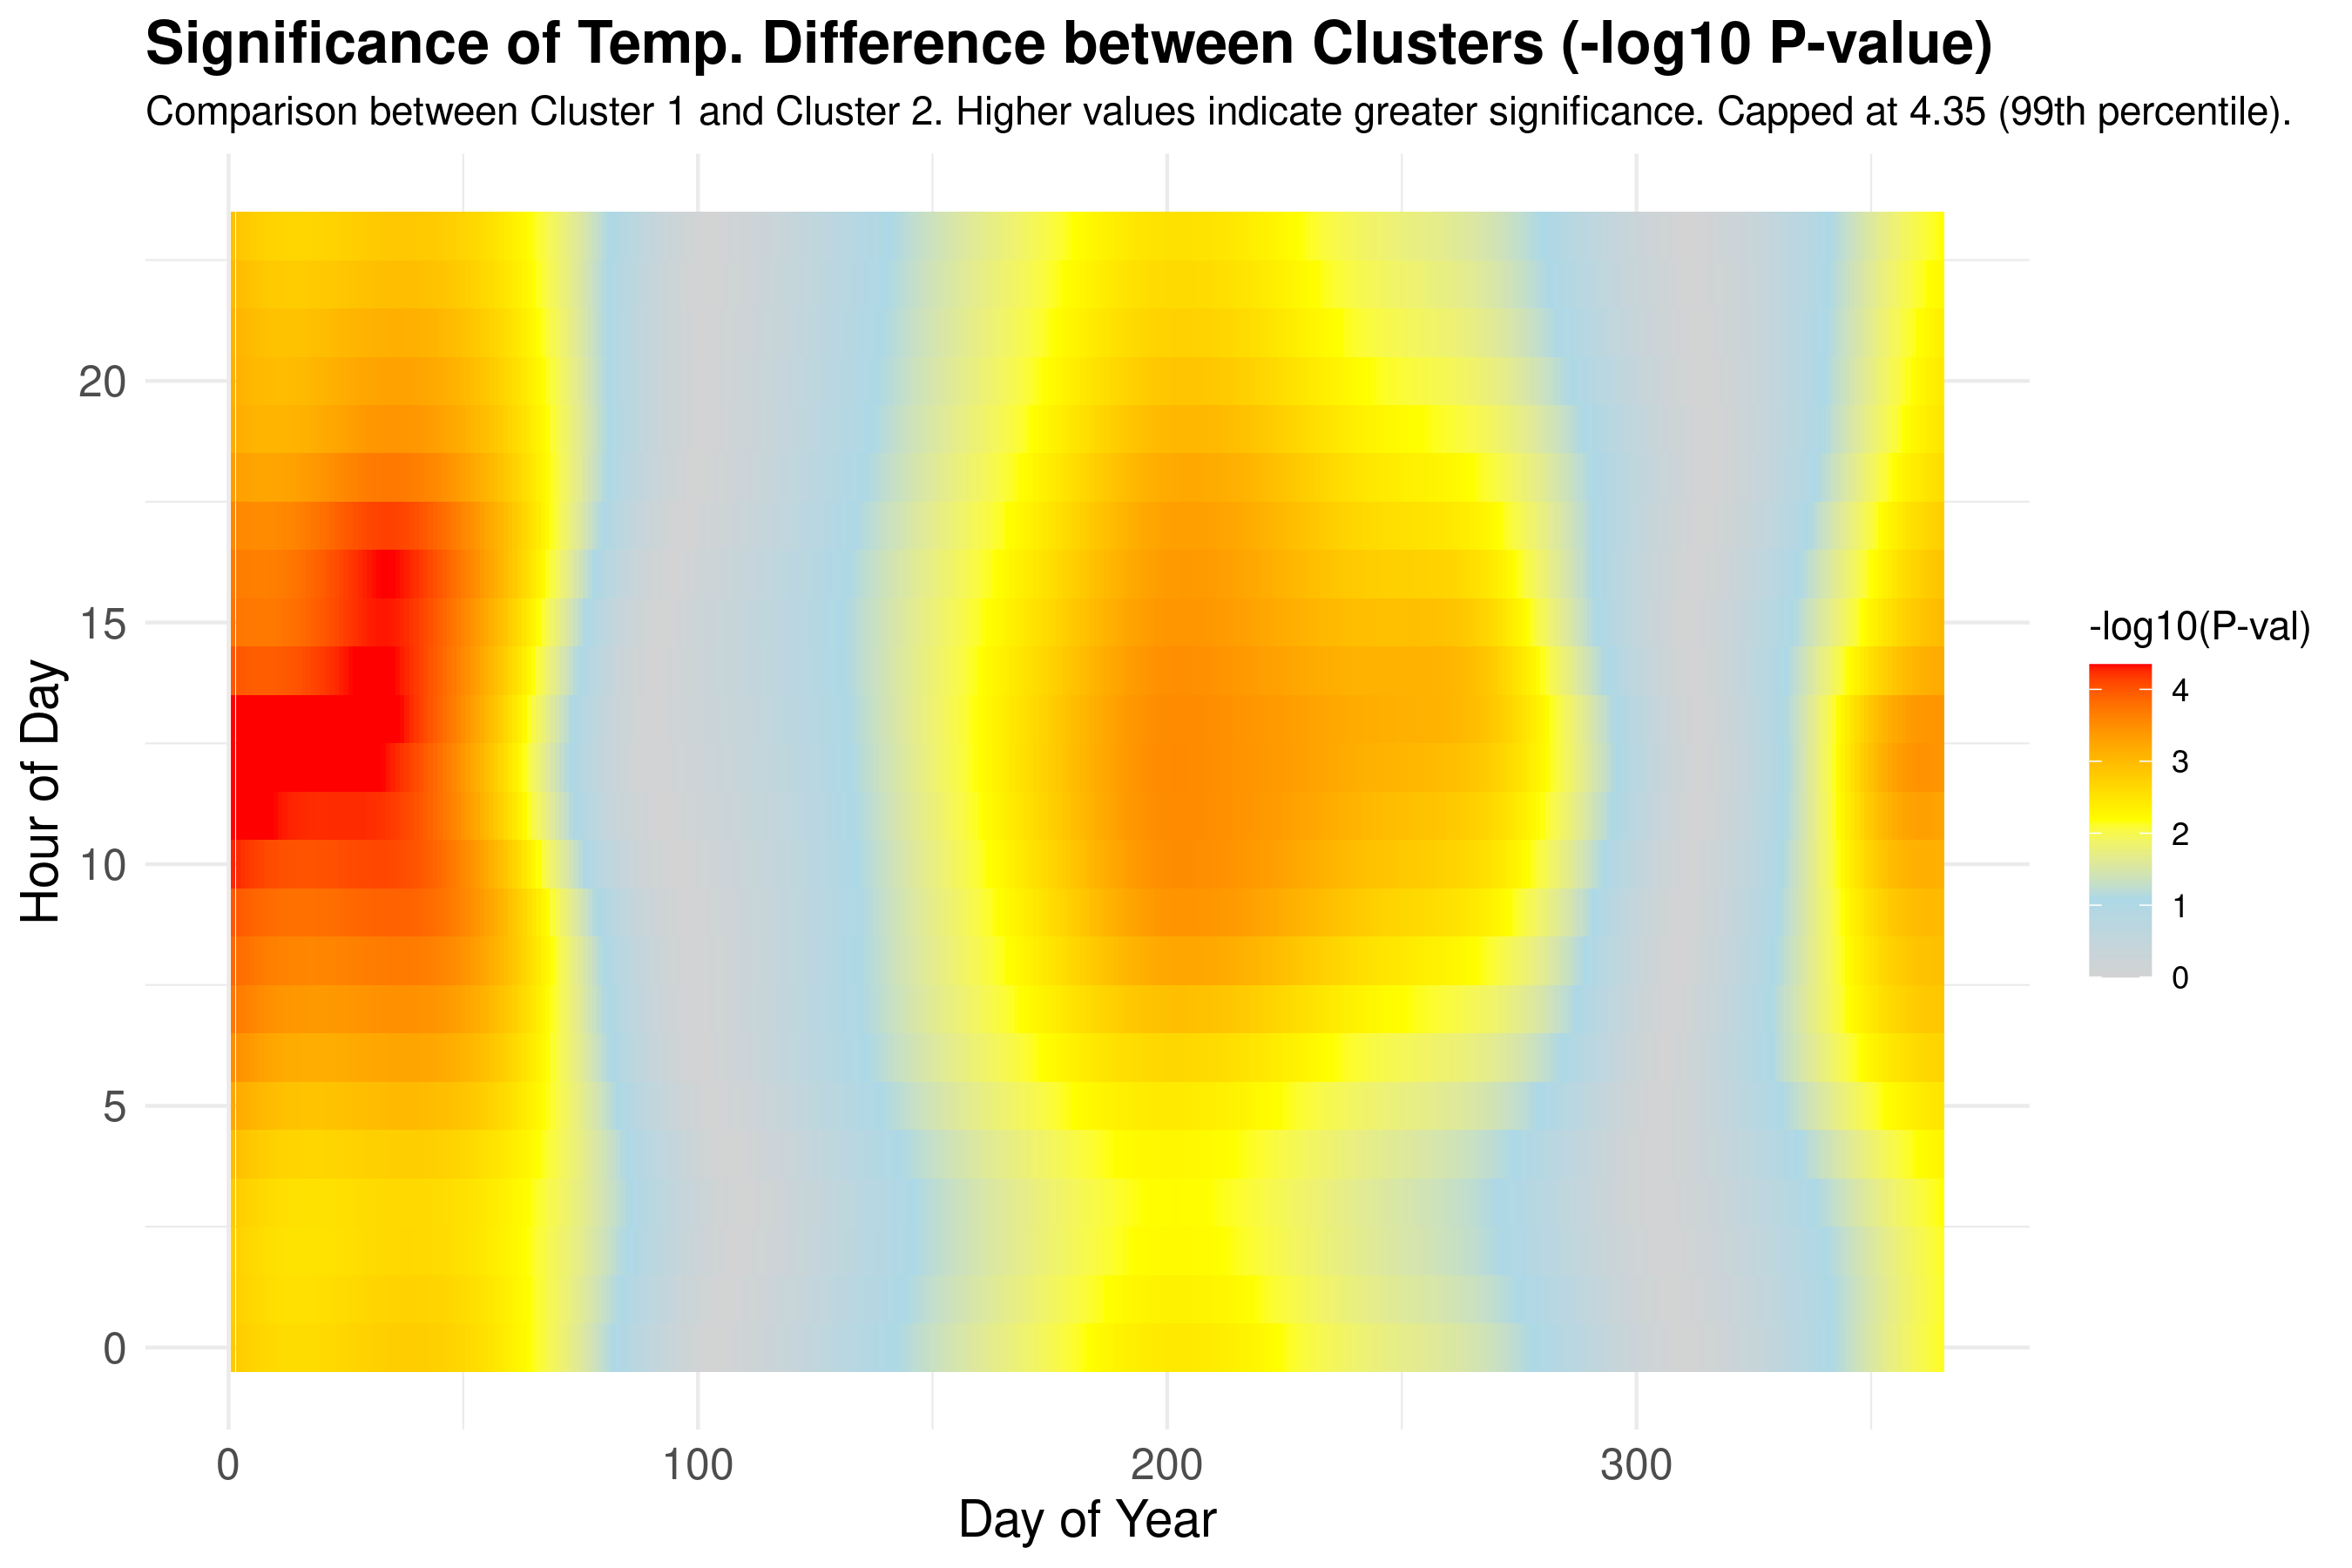
\includegraphics[width=0.85\linewidth]{../data/output/figures/pointwise_anova_clusters_heatmap.png}
    \caption{Higher values indicate stronger statistical significance of temperature difference between clusters. Red line ($-\log_{10}(0.05) \approx 1.3$) indicates p=0.05 threshold.}
  \end{figure}
  \textbf{Interpretation:}
  \begin{itemize}
    \item \textbf{Significant Differences (Yellow/Orange/Red areas):}
        \begin{itemize}
            \item Primarily during winter months (Days $\sim$0-60 and $\sim$300-365) across most hours.
            \item Also during peak summer daytimes (Days $\sim$120-180, around midday).
        \end{itemize}
    \item \textbf{Less Significant Differences (Light Blue/Grey areas):}
        \begin{itemize}
            \item During transitional seasons or periods where temperature profiles are more similar.
        \end{itemize}
    \item This confirms that the visual differences in mean cluster surfaces are statistically significant at specific times of the year and day.
  \end{itemize}
\end{frame}


% --- CONCLUSION ---
\section{Conclusion}
\begin{frame}{Conclusions and Future Work}
  \textbf{Key Findings from Advanced FDA:}
  \begin{itemize}
    \item \textbf{Derivatives \& Covariance:} Revealed detailed intra-day and inter-day temperature dynamics and relationships.
    \item \textbf{Yearly FPCA:} Quantified inter-annual variability and highlighted distinct city-level climatic trajectories over the years.
    \item \textbf{Clustering:} Successfully grouped cities into geographically and climatically meaningful clusters based on their annual temperature surfaces.
        \begin{itemize}
            \item Cluster 1: Southern/Central cities with milder variations.
            \item Cluster 2: Northern cities with more extreme seasonal variations.
        \end{itemize}
    \item \textbf{Pointwise FANOVA:} Confirmed statistically significant differences in temperature patterns between clusters, particularly during winter and peak summer daytimes.
  \end{itemize}
  \pause
  \textbf{Potential Future Work:}
  \begin{itemize}
    \item Incorporate other meteorological variables (humidity, precipitation) into a multivariate FDA.
    \item Functional regression models (e.g., predicting energy demand based on temperature curves).
    \item Anomaly detection for unusual yearly temperature patterns.
    \item Explore more sophisticated clustering methods or different numbers of clusters.
  \end{itemize}
\end{frame}

\begin{frame}{Thank You!}
	\begin{center}
		\Huge Thank you for your attention!
	\end{center}
\end{frame}

\end{document}
